\documentclass{article}
\usepackage[utf8]{inputenc}
\usepackage[a4paper,top=1.5cm,bottom=1.5cm,left=3cm,right=3cm,marginparwidth=1.75cm]{geometry}
\usepackage{natbib}
\usepackage{graphicx}
\usepackage{amsmath, amsthm, amssymb, amsfonts}
\usepackage{titlesec}
\usepackage{makecell}
\usepackage{inconsolata}
\usepackage{tikz}
\usepackage{caption, copyrightbox}
\captionsetup{justification=centering, labelfont=sc, labelsep=endash}
\usepackage{minted}
\usetikzlibrary{automata,positioning}
\usetikzlibrary{arrows}
\usetikzlibrary{shapes}
\definecolor{blue(pigment)}{rgb}{0.2, 0.2, 0.6}
\definecolor{blue(ryb)}{rgb}{0.01, 0.28, 1.0}
\definecolor{brightcerulean}{rgb}{0.11, 0.67, 0.84}
\definecolor{emerald}{rgb}{0.31, 0.78, 0.47}
\tikzset {
        recnode/.style={align=center,inner sep=0pt, rectangle, text width=5cm, draw,thick,minimum width=5cm,minimum height=1cm},
        default/.style={}
}
\usepackage{nicematrix}
\usepackage{multirow}

\makeatletter
\@addtoreset{subsection}{section}
\@addtoreset{subsection}{*section}
\makeatother
\def\thesubsection{\arabic{subsection}}

\let\oldsection\section
\renewcommand{\section}{%
    \setcounter{subsection}{0}%
    \oldsection%
}


\title{Computer Networks - HW2}
\author{Alireza Rostami \\ Student Number: 9832090}
\date{}

\begin{document}
    \maketitle
    
    \section*{Question 1}
    The propagation speed is $2.5 \times 10^{8} \, \frac{m}{s}$. The distance is $2500 km \equiv 2.5 \times 10^6 \, m$. Therefore, we divide the latter by the former, we would left with time, which is the propagation time.
    \begin{displaymath}
        \frac{2.5 \times 10^{6} \, \frac{m}{s}}{2.5 \times 10^8 \, m} = 10 \, ms
    \end{displaymath}
    
    ~\\As you can see it does not depend on neither packet length nor transmission rate.
    
    ~\\More generally, the formula is given as:
    \begin{displaymath}
        t = \frac{d}{s}
    \end{displaymath}

    \section*{Question 2}
Suppose \textsl{system A} want to sent packet to \textsl{system B}. Steps involved in this process are given below:
\begin{enumerate}
    \item System A first breaks large file into small pieces named \textsl{chunks}.
    \item It adds separate headers for each chunks so that each chunk appers like separate packet.
    \item Header file in chunks contain IP address of receiver; here, \textsl{system B}.
    \item Switch system uses IP present in header to determine link to destination.
\end{enumerate}
When we travel from one city to another and we do not know the path, we would ask for path and go on that. Which is analogous to the switching process.
\newpage
\section*{Question 3}
    \begin{center}
        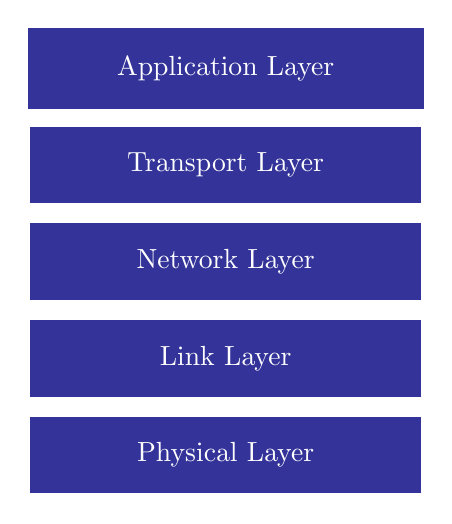
\begin{tikzpicture}[every node/.style=recnode]
            \node[white, draw=blue(pigment), fill=blue(pigment)] (ApplicationLayer) at (0,0) {
                Application Layer
            };
            \node[below=2mm of ApplicationLayer, white, fill=blue(pigment), fill=blue(pigment)] (TransportLayer) {
                Transport Layer
            };
            \node[below=2mm of TransportLayer, white, fill=blue(pigment), fill=blue(pigment)] (NetworkLayer) {
                Network Layer
            };
            \node[below=2mm of NetworkLayer, white, fill=blue(pigment), fill=blue(pigment)] (DataLinkLayer) {
                Link Layer
            };
            \node[below=2mm of DataLinkLayer, white, fill=blue(pigment), fill=blue(pigment)] (PhysicalLayer) {
                Physical Layer
            };
        \end{tikzpicture}
    \end{center}
    \subsection{Application Layer}
The application layer is responsible for communication between applications running on two different end systems. A message or data transferred from one end is readable for the corresponding application on the other end. These applications include web browsers, email clients, etc.

    
    \subsection{Transport Layer}
On the sending end, the transport layer is responsible for collecting the application layer message from the relevant end-point and transferring it to the network layer to be communicated over the network. The receiving end collects the message from the network layer and passes it on to the relevant end-point where the application layer can access that message.

    \subsection{Network Layer}
The network layer is responsible for transferring data from one system to another on the network. The transport layer passes a segment and the destination address to the network layer. Then, it is the responsibility of the network layer to transfer the data to the destination end-system over the network. This layer also takes care of the routing of data on intermediate routers.


    \subsection{Link Layer}
When a packet is being transferred over the internet, several intermediate devices are between the two end systems. These devices may be routers, switches, or other computers. The link layer is responsible for communication between one device and its immediate neighbor. The link-layer is mostly implemented in technologies like ethernet, Wi-Fi, token ring, etc.




    \subsection{Physical Layer}
The physical layer is responsible for breaking the data frame into bits, converting it into a form that can be transmitted over the physical communication line, and transferring it. This form could be light pulses (fiber-optic), radio waves (for wireless communication, or electric pulses (for wired communication). On the receiving end, the physical layer collects the stream of bits and reassembles it into a data frame that is then passed onto the link layer for further processing.

\section*{Question 4} The IP address of the destination host and the port number of the destination socket.
\newpage

\section*{Question 5} The address \texttt{10.10.10.0/24} is in prefix format. We can deduce the subnet mask format as:

\begin{displaymath}
    \text{IP: }\texttt{10.10.10.0}
\end{displaymath}
\begin{displaymath}
    \text{Subnet mask: }\texttt{255.255.255.0}
\end{displaymath}

To have eight subnets, we need $\log_2 8 = 3$ bits. With respect to the subnet mask, we use the fourth octet to achieve this.
\begin{table}[h!]
\centering
\begin{tabular}{|c|c|c|c|c|}
\hline
& First octet (Dec.) & Second octet (Dec.) & Third octet (Dec.) & Fourth octet (Bin.) \\ \hline
Original IP & 10 & 10 & 10 & 00000000 \\
Subnet 0 & 10 & 10 & 10 & 00000000 \\
Subnet 1 & 10 & 10 & 10 & 00100000 \\
Subnet 2 & 10 & 10 & 10 & 01000000 \\
Subnet 3 & 10 & 10 & 10 & 01100000 \\
Subnet 4 & 10 & 10 & 10 & 10000000 \\
Subnet 5 & 10 & 10 & 10 & 10100000 \\
Subnet 6 & 10 & 10 & 10 & 11000000 \\
Subnet 7 & 10 & 10 & 10 & 11100000 \\ \hline
\end{tabular}
\end{table}
~\\The new subnet mask would become: \texttt{255.255.255.11100000} which is \texttt{255.255.255.224}.

~\\The network ID of each subnet is the address of is:
\begin{table}[h!]
\centering
\begin{tabular}{|c|c|c|c|c|c|}
\hline
& First octet & Second octet & Third octet & Fourth octet (Bin.) & ID \\ \hline
Subnet 0 & 10 & 10 & 10 & 00000000 & 10.10.10.0 \\
Subnet 1 & 10 & 10 & 10 & 00100000 & 10.10.10.32 \\
Subnet 2 & 10 & 10 & 10 & 01000000 & 10.10.10.64 \\
Subnet 3 & 10 & 10 & 10 & 01100000 & 10.10.10.96\\
Subnet 4 & 10 & 10 & 10 & 10000000 & 10.10.10.128\\
Subnet 5 & 10 & 10 & 10 & 10100000 & 10.10.10.160 \\
Subnet 6 & 10 & 10 & 10 & 11000000 & 10.10.10.192\\
Subnet 7 & 10 & 10 & 10 & 11100000 & 10.10.10.224 \\ \hline
\end{tabular}
\end{table}

~\\ The broadcast ID of each subnet is:
\begin{table}[h!]
\centering
\begin{tabular}{|c|c|c|c|c|c|}
\hline
& First octet & Second octet & Third octet & Fourth octet (Bin.) & ID \\ \hline
Subnet 0 & 10 & 10 & 10 & 00011111 & 10.10.10.31 \\
Subnet 1 & 10 & 10 & 10 & 00111111 & 10.10.10.63 \\
Subnet 2 & 10 & 10 & 10 & 01011111 & 10.10.10.95 \\
Subnet 3 & 10 & 10 & 10 & 01111111 & 10.10.10.127\\
Subnet 4 & 10 & 10 & 10 & 10011111 & 10.10.10.159\\
Subnet 5 & 10 & 10 & 10 & 10111111 & 10.10.10.191 \\
Subnet 6 & 10 & 10 & 10 & 11011111 & 10.10.10.223\\
Subnet 7 & 10 & 10 & 10 & 11111111 & 10.10.10.255 \\ \hline
\end{tabular}
\end{table}
\newpage

\section*{Question 6} We can deduce from the class A network ID the subnet mask format as:
\begin{displaymath}
    \text{Subnet mask: }\texttt{255.0.0.0}
\end{displaymath}

To have eight subnets, we need $\log_2 8 = 3$ bits. With respect to the subnet mask, we use the second octet to achieve this.
\begin{table}[h!]
\centering
\begin{tabular}{|c|c|c|c|c|}
\hline
& First octet (Dec.) & Second octet (Bin.) & Third octet (Dec.) & Fourth octet (Dec.) \\ \hline
Original IP & 14 & 00000000 & 0 & 0 \\
Subnet 0 & 14 & 00000000 & 0 & 0 \\
Subnet 1 & 14 & 00100000 & 0 & 0 \\
Subnet 2 & 14 & 01000000 & 0 & 0 \\
Subnet 3 & 14 & 01100000 & 0 & 0 \\
Subnet 4 & 14 & 10000000 & 0 & 0 \\
Subnet 5 & 14 & 10100000 & 0 & 0 \\
Subnet 6 & 14 & 11000000 & 0 & 0 \\
Subnet 7 & 14 & 11100000 & 0 & 0 \\ \hline
\end{tabular}
\end{table}
~\\The new subnet mask would become: \texttt{255.11100000.0.0} which is \texttt{255.224.0.0}.

~\\The network ID of each subnet is the address of is:
\begin{table}[h!]
\centering
\begin{tabular}{|c|c|c|c|c|c|}
\hline
& First octet & Second octet (Bin.) & Third octet & Fourth octet & ID \\ \hline
Subnet 0 & 14 & 00000000 & 0 & 0 & 14.0.0.0 \\
Subnet 1 & 14 & 00100000 & 0 & 0 & 14.32.0.0 \\
Subnet 2 & 14 & 01000000 & 0 & 0 & 14.64.0.0 \\
Subnet 3 & 14 & 01100000 & 0 & 0 & 14.96.0.0\\
Subnet 4 & 14 & 10000000 & 0 & 0 & 14.128.0.0\\
Subnet 5 & 14 & 10100000 & 0 & 0 & 14.160.0.0 \\
Subnet 6 & 14 & 11000000 & 0 & 0 & 14.192.0.0\\
Subnet 7 & 14 & 11100000 & 0 & 0 & 14.224.0.0 \\ \hline
\end{tabular}
\end{table}

~\\The first valid address of each subnet is:
\begin{table}[h!]
\centering
\begin{tabular}{|c|c|c|c|c|c|}
\hline
& First octet & Second octet (Bin.) & Third octet & Fourth octet & ID \\ \hline
Subnet 0 & 14 & 00000000 & 0 & 1 & 14.0.0.1 \\
Subnet 1 & 14 & 00100000 & 0 & 1 & 14.32.0.1 \\
Subnet 2 & 14 & 01000000 & 0 & 1 & 14.64.0.1 \\
Subnet 3 & 14 & 01100000 & 0 & 1 & 14.96.0.1\\
Subnet 4 & 14 & 10000000 & 0 & 1 & 14.128.0.1\\
Subnet 5 & 14 & 10100000 & 0 & 1 & 14.160.0.1 \\
Subnet 6 & 14 & 11000000 & 0 & 1 & 14.192.0.1\\
Subnet 7 & 14 & 11100000 & 0 & 1 & 14.224.0.1 \\ \hline
\end{tabular}
\end{table}


~\\ The broadcast ID of each subnet is:
\begin{table}[h!]
\centering
\begin{tabular}{|c|c|c|c|c|c|}
\hline
& First octet & Second octet (Bin.) & Third octet & Fourth octet & ID \\ \hline
Subnet 0 & 14 & 00011111 & 255 & 255 & 14.31.255.255 \\
Subnet 1 & 14 & 00111111 & 255 & 255 & 14.63.255.255 \\
Subnet 2 & 14 & 01011111 & 255 & 255 & 14.95.255.255 \\
Subnet 3 & 14 & 01111111 & 255 & 255 & 14.127.255.255\\
Subnet 4 & 14 & 10011111 & 255 & 255 & 14.159.255.255\\
Subnet 5 & 14 & 10111111 & 255 & 255 & 14.191.255.255 \\
Subnet 6 & 14 & 11011111 & 255 & 255 & 14.223.255.255\\
Subnet 7 & 14 & 11111111 & 255 & 255 & 14.255.255.255 \\ \hline
\end{tabular}
\end{table}

~\\ The last valid address of each subnet is:
\begin{table}[h!]
\centering
\begin{tabular}{|c|c|c|c|c|c|}
\hline
& First octet & Second octet (Bin.) & Third octet & Fourth octet & ID \\ \hline
Subnet 0 & 14 & 00011111 & 255 & 254 & 14.31.255.254 \\
Subnet 1 & 14 & 00111111 & 255 & 254 & 14.63.255.254 \\
Subnet 2 & 14 & 01011111 & 255 & 254 & 14.95.255.254 \\
Subnet 3 & 14 & 01111111 & 255 & 254 & 14.127.255.254\\
Subnet 4 & 14 & 00011111 & 255 & 254 & 14.159.255.254 \\
Subnet 5 & 14 & 00111111 & 255 & 254 & 14.191.255.254 \\
Subnet 6 & 14 & 01011111 & 255 & 254 & 14.233.255.254 \\
Subnet 7 & 14 & 01111111 & 255 & 254 & 14.255.255.254\\ \hline


\end{tabular}
\end{table}
\newpage

\section*{Question 7} We can deduce from the class B network ID the subnet mask format as:
\begin{displaymath}
    \text{Subnet mask: }\texttt{255.255.0.0}
\end{displaymath}
The offset is given as 16.
\begin{table}[h!]
\centering
\begin{tabular}{|c|c|c|c|c|}
\hline
& First octet (Dec.) & Second octet (Dec.) & Third octet (Bin.) & Fourth octet (Dec.) \\ \hline
Original IP & 150 & 87 & 00000000 & 0 \\
Subnet 0 & 150 & 87 & 00000000 & 0 \\
Subnet 1 & 150 & 87 & 00010000 & 0 \\
Subnet 2 & 150 & 87 & 00100000 & 0 \\
Subnet 3 & 150 & 87 & 00110000 & 0 \\
Subnet 4 & 150 & 87 & 01000000 & 0 \\
Subnet 5 & 150 & 87 & 01010000 & 0 \\ \hline

\end{tabular}
\end{table}
~\\The new subnet mask would become: \texttt{255.255.11110000.0} which is \texttt{255.255.240.0}.

~\\The network ID of each subnet is the address of is:
\begin{table}[h!]
\centering
\begin{tabular}{|c|c|c|c|c|c|}
\hline
& First octet & Second octet & Third octet (Bin.) & Fourth octet & ID \\ \hline
Subnet 0 & 150 & 87 & 00000000 & 0 & 150.87.0.0 \\
Subnet 1 & 150 & 87 & 00010000 & 0 & 150.87.16.0 \\
Subnet 2 & 150 & 87 & 00100000 & 0 & 150.87.32.0 \\
Subnet 3 & 150 & 87 & 00110000 & 0 & 150.87.48.0\\
Subnet 4 & 150 & 87 & 01000000 & 0 & 150.87.64.0\\
Subnet 5 & 150 & 87 & 01010000 & 0 & 150.87.80.0\\ \hline

\end{tabular}
\end{table}

~\\The first valid address of each subnet is:
\begin{table}[h!]
\centering
\begin{tabular}{|c|c|c|c|c|c|}
\hline
& First octet & Second octet & Third octet (Bin.) & Fourth octet & ID \\ \hline
Subnet 0 & 150 & 87 & 00000000 & 1 & 150.87.0.1 \\
Subnet 1 & 150 & 87 & 00010000 & 1 & 150.87.16.1 \\
Subnet 2 & 150 & 87 & 00100000 & 1 & 150.87.32.1 \\
Subnet 3 & 150 & 87 & 00110000 & 1 & 150.87.48.1\\
Subnet 4 & 150 & 87 & 01000000 & 1 & 150.87.64.1\\
Subnet 5 & 150 & 87 & 01010000 & 1 & 150.87.80.1\\ \hline
\end{tabular}
\end{table}


~\\ The broadcast ID of each subnet is:
\begin{table}[h!]
\centering
\begin{tabular}{|c|c|c|c|c|c|}
\hline
& First octet & Second octet & Third octet (Bin.) & Fourth octet & ID \\ \hline
Subnet 0 & 150 & 87 & 00001111 & 255 & 150.87.15.255 \\
Subnet 1 & 150 & 87 & 00011111 & 255 & 150.87.31.255 \\
Subnet 2 & 150 & 87 & 00101111 & 255 & 150.87.47.255 \\
Subnet 3 & 150 & 87 & 00111111 & 255 & 150.87.63.255 \\
Subnet 4 & 150 & 87 & 01001111 & 255 & 150.87.79.255 \\
Subnet 5 & 150 & 87 & 01011111 & 255 & 150.87.95.255 \\ \hline
\end{tabular}
\end{table}


~\\ The last valid address of each subnet is:
\begin{table}[h!]
\centering
\begin{tabular}{|c|c|c|c|c|c|}
\hline
& First octet & Second octet & Third octet (Bin.) & Fourth octet & ID \\ \hline
Subnet 0 & 150 & 87 & 00001110 & 254 & 150.87.15.254 \\
Subnet 1 & 150 & 87 & 00011110 & 254 & 150.87.31.254 \\
Subnet 2 & 150 & 87 & 00101110 & 254 & 150.87.47.254 \\
Subnet 3 & 150 & 87 & 00111110 & 254 & 150.87.63.254 \\
Subnet 4 & 150 & 87 & 01001110 & 254 & 150.87.79.254 \\
Subnet 5 & 150 & 87 & 01011110 & 254 & 150.87.95.254 \\ \hline
\end{tabular}
\end{table}

\newpage

\section*{Question 8} We can deduce from the class B network ID the subnet mask format as:
\begin{displaymath}
    \text{Subnet mask: }\texttt{255.255.0.0}
\end{displaymath}
To have four subnets, we need $\log_2 4 = 2$ bits. With respect to the subnet mask, we use the third octet to achieve this.
\begin{table}[h!]
\centering
\begin{tabular}{|c|c|c|c|c|}
\hline
& First octet (Dec.) & Second octet (Dec.) & Third octet (Bin.) & Fourth octet (Dec.) \\ \hline
Original IP & 141 & 85 & 00000000 & 0 \\
Subnet 0 & 141 & 85 & 00000000 & 0 \\
Subnet 1 & 141 & 85 & 01000000 & 0 \\
Subnet 2 & 141 & 85 & 10000000 & 0 \\
Subnet 3 & 141 & 85 & 11000000 & 0 \\ \hline
\end{tabular}
\end{table}
~\\The new subnet mask would become: \texttt{255.255.11000000.0} which is \texttt{255.255.192.0}.

~\\The network ID of each subnet is the address of is:
\begin{table}[h!]
\centering
\begin{tabular}{|c|c|c|c|c|c|}
\hline
& First octet & Second octet & Third octet (Bin.) & Fourth octet & ID \\ \hline
Subnet 0 & 141 & 85 & 00000000 & 0 & 141.85.0.0 \\
Subnet 1 & 141 & 85 & 01000000 & 0 & 141.85.64.0 \\
Subnet 2 & 141 & 85 & 10000000 & 0 & 141.85.128.0 \\
Subnet 3 & 141 & 85 & 11000000 & 0 & 141.85.192.0\\ \hline
\end{tabular}
\end{table}

~\\ The broadcast ID of each subnet is:
\begin{table}[h!]
\centering
\begin{tabular}{|c|c|c|c|c|c|}
\hline
& First octet & Second octet & Third octet (Bin.) & Fourth octet & ID \\ \hline
Subnet 0 & 141 & 85 & 00111111 & 255 & 141.85.63.255 \\
Subnet 1 & 141 & 85 & 01111111 & 255 & 141.85.127.255 \\
Subnet 2 & 141 & 85 & 10111111 & 255 & 141.85.191.255 \\
Subnet 3 & 141 & 85 & 11111111 & 255 & 141.85.255.255\\ \hline
\end{tabular}
\end{table}


\end{document}
